\documentclass[12pt]{article}
\usepackage[letterpaper, margin=1in]{geometry}
\usepackage{amsmath,amssymb,amsthm,amsfonts}
\usepackage[version=4]{mhchem}
\usepackage{mathtools}
\usepackage[utf8]{inputenc}
\usepackage[english]{babel}
\usepackage{titlesec} 

\newcommand{\ug}{uG4\xspace}
\newcommand{\delT}[1]{\frac{\partial #1}{\partial t}}
\newcommand{\ccyt}[0]{c_c}
\newcommand{\cer}[0]{c_e}
\newcommand{\ip}[1]{p}
\newcommand{\cca}[0]{[\mathrm{Ca}^{2+}]}
\newcommand{\cip}[0]{[\mathrm{IP}_3]}

\renewcommand{\baselinestretch}{1.125}



\titleformat{\subsection}[runin]
  {\normalfont\normalsize\bfseries}{\thesubsection}{2em}{}

\titleformat{\subsubsection}[runin]
  {\normalfont\normalsize\itshape}{\thesubsubsection}{2em}{}

%\title{An Ultrastructural study on the effects of Neuron Calcium Dynamics under Transcranial Magnetic Stimulation }
\title{Ultrastructural Neuronal Modeling of Calcium Dynamics under Transcranial Magnetic Stimulation}
\author{James Rosado}
%\date{March 2021}

\begin{document}

\maketitle

\section{Introduction}
 An important question in the study of calcium (Ca$^{2+}$) signaling is how this ion regulates a wide spectrum of cellular processes, which include: fertilization, proliferation, learning, and cell death, all of which are the result of synaptic strengthening/weakening. Part of the answer lies in the spatial-temporal interactions of Ca$^{2+}$ at the extracellular and intracellular levels of a neuron \cite{SMEDLER2014964}. There is a complex concert of Ca$^{2+}$ ion exchange and transport mechanisms that are activated (or inactivated) by external stimuli and it remains to be studied the role of these interactions at the ultrastructural scale. \\
\indent One mode of external stimulation is by Transcranial Magnetic Stimulation (TMS) and repetitive TMS (rTMS). TMS is a noninvasive brain stimulation method to modulate human brain activity by generating a strong magnetic field near the cranium  \cite{Barker1985}. The magnetic field traverses the skull to induce an electric field which may depolarize neurons \cite{Hallett2007}; therefore, TMS is used in clinical applications to treat neuropsychiatric and neurological disorders \cite{Lefaucheur2014}. However, it is not well known the affects of TMS on intracellular Ca$^{2+}$ interactions; therefore, we endeavor to determine the types of calcium interactions that occur when a neuron experiences TMS.  \\
\indent %In addition to studying the effects of TMS/rTMS on calcium ions, 
We also determine how intracellular calcium mechanisms are affected by TMS stimuli. In particular, the cellular regulators of calcium are given by: the internal Ca$^{2+}$ store (``calcium bank'') of a neuron called the endoplasmic reticulum (ER) with spine apparatus (SA), the voltage dependent calcium channels (VDCCs), and calcium influx at synaptic spines. %Synaptic spines are protrusions from dendrites which form contacts with chemically connected cells, they are the location of the SA.
%an example of a 3D-reconstructed spine is shown in figure \ref{spinedend}. The spine-interior often contains an organelle, the spine apparatus (SA) shown in figure \ref{spinedend}B)-\ref{spinedend}D), which is a continuous extension of ER in the dendrite. 
Ultimately, the ER is responsible for synaptic plasticity \cite{Breit2018} and from here we determine under what conditions does TMS cause intracellular calcium to induce synaptic plasticity.
% (either increase or decrease) by affecting the intracellular calcium interactions.
%\begin{figure}[ht!]
%    \centering
%    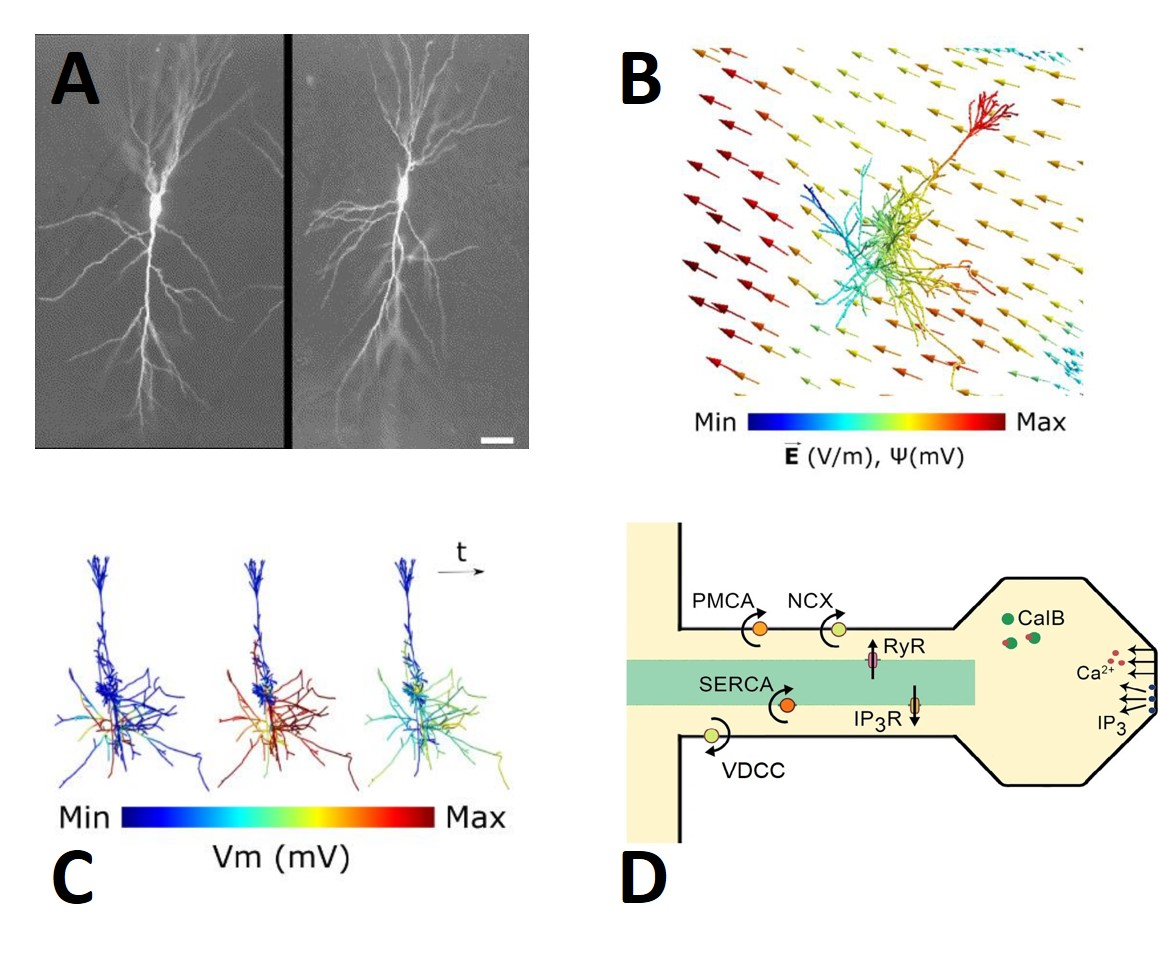
\includegraphics[width=0.75\linewidth]{images/Picture2.jpg}
%    \caption{A) These are image reconstructions of pyramidal neurons \cite{SANTOS2004481}, B) this shows a pyramidal neuron experiencing an electric field \cite{Shirinpour2020.09.23.310219}, C) shows the same cells change in PM voltage, and D) schematic drawing of the PM transport mechanisms and intracellular mechanisms \cite{BreitKessler2018}}
%    \label{fig:picture2}
%\end{figure}

\section{Statement of Research}
\subsection*{Research Objectives}
For this project I endeavor to formulate a spatio-temporal calcium methodology which will predict when a calcium wave is initiated by ion exchanges due to: the intracellular mechanisms  SA and ER, PM transport mechanisms (including VDCCs), and extracellular effects i.e. electric fields and post synaptic calcium influx. The methodology takes into account the aforementioned physiological phenomena, and will determine geometric properties of the PM, ER, SA, and electric field under which a calcium wave is propagated through the dendrite.% enough to induce firing of an action potential from the soma.

This project requires detailed simulations of surface and volumetric geometries. The degrees of freedom (DoFs) of the geometries can range from $10^6-10^9$ depending on the scope of the geometry i.e. spine-dendrite simulations to full cell simulations. The simulation times can range from 30 ms to 3 seconds; in particular, 30 ms simulations are used to determine the physiological parameters of the SA for which  calcium enters the dendritic region of the neuron. Longer simulations in the 1-3 second range are used to determine the stability of the calcium wave(s) that are propagated.
%these simulations may require a longer end time in order for a calcium wave to reach the soma.

Some of the physiological parameters studied in the project are ryandoine-receptor (RyR) density, initial Ca$^{2+}$ concentration, IP3R density, post synaptic calcium influx, and ER calcium concentration. For the simulations I will run parameter sweeps of each of the physiological values i.e. run a simulation where the RyR density is incremented by 0.01. Geometric parameters are also taken into account such as SA volume, synapse area, spine surface area and volume, electric field orientation, electric field intensity; all of which are used to determine correlations of the physiological parameters.
The model equations are simulated on three types of spine geometries: neck, mushroom, and stubby spines.
%I am running these simulations on 9 spines and SA that were reconstructed in 3D from the Vlachos Lab; these spines/SA represent a range of the different qualitative types of spine-dendrites that are observed i.e. neck, mushroom, and stubby spines.
To summarize, my objective is to establish novel methodologies for strengthening neuron calcium signaling under given physiological conditions by determining
\begin{itemize}
    \item [a)] empirical laws that predict a release of calcium into the dendrite volume region,
    \item [b)] minimal ER/SA geometric properties and TMS/rTMS induced electrical field properties that allow stable calcium wave propagation.
\end{itemize}
%\begin{itemize}
    %\item[1)] Establish a novel methodology for strengthening neuron calcium signaling under given physiological conditions by
 %   \item [1)] Determine empirical laws that predict a release of calcium into the dendrite volume region.
  %  \item[2)] Determine minimal ER/SA geometric properties and electric field properties that allow stable propagation of calcium through a section of dendrite.
    %\item[3)] Derive a model from 1) and 2) and study and predict the nature of calcium propagation at the full cell level.
   % \item[4)] Use the model to determine the affect TMS has on calcium propagation.
%\end{itemize}
%\begin{figure}[ht!]
%    \centering
%    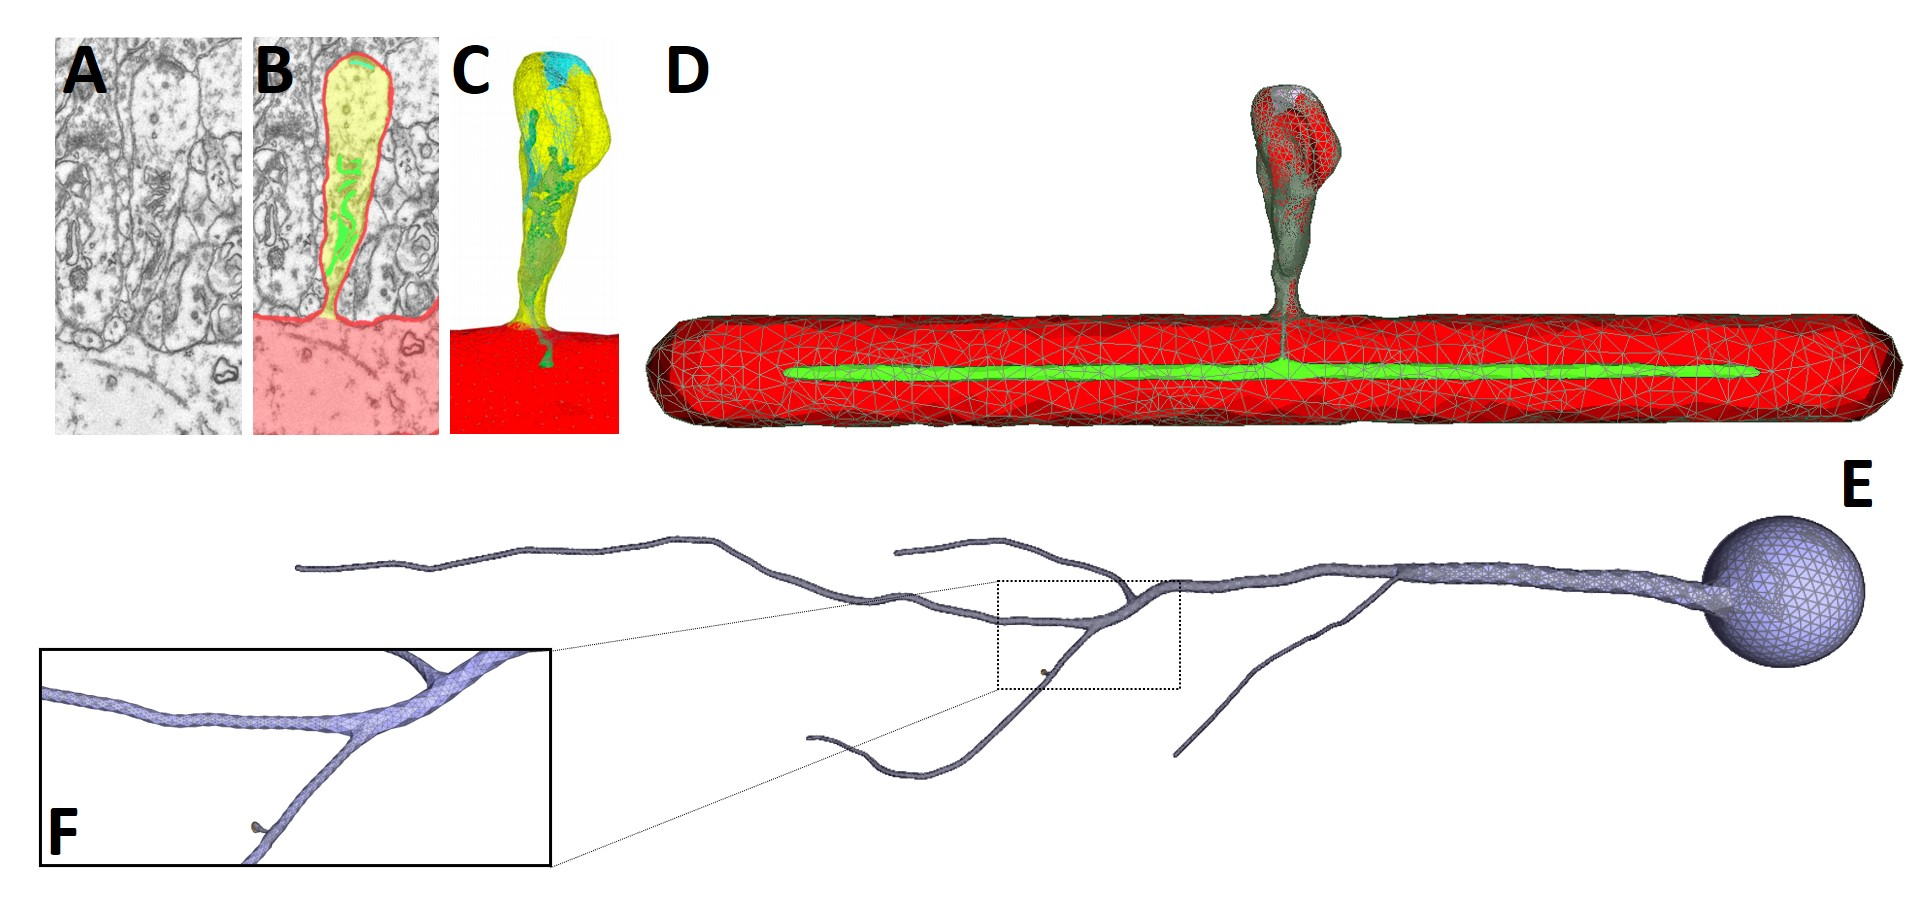
\includegraphics[width=\linewidth]{images/Picture1.jpg}
%    \caption{A) The spine-dendrite image data is collected under microscopy, B) image segmentation is used to capture the contours of the morphology, C) a 3D geometry constructed. And for D) we run simulations on a segment of cylindrical dendrite, and then E),F) we position the spine-dendrite on an full cell geometry to perform our simulations. For D)-F) we process the geometries by tetrahedralizing the surface meshes}
%    \label{spinedend}
%\end{figure}

%\subsection*{Modeling TMS} TMS induced electric fields are calculated using FEM models implemented in the open-source software SimNIBS v3.1 \cite{Saturnino2019}. The equations that govern the electric field $E$ caused by a TMS coil are given by \cite{WeipingWang1994}
%\begin{align*}
%    \nabla \cdot (\sigma\nabla\phi) &= -\nabla\cdot\left(\sigma \frac{\partial A}{\partial t}\right)\\
%    E &= -\nabla\phi -\frac{\partial A}{\partial t}
%\end{align*}
%where $\sigma$ is the tissue-specific ohmic conductivity, $A$ is the magnetic vector potential of the TMS coil, and $\phi$ is the electrical potential from a secondary source of electric field caused by variations in tissue conductivities. 
%For the simulations we will assume a quasi-static assumption, that is the time course of the TMS electric field is identical to the TMS stimulation, i.e. rate of change of the coil current $\frac{dI}{dt}$. Once the TMS electric field is computed, then the $E$-field is coupled with the neuron model using Yale Neuron. From the Yale Neuron framework, we obtain TMS voltage traces that are induced on the cell membrane and the voltage trace data is then used in the calcium simulations, i.e. to study the calcium release patterns of voltage-dependent calcium channels (VDCCs). The VDCCs are described by the model from \cite{BorgGraham1999}.
%\subsection*{Model Equations for Calcium Dynamics}
%Three-dimensional spatio-temporal Ca$^{2+}$ and inositol %trisphosphate (IP3) dynamics in
%the intracellular space are modeled by a system of diffusion-reaction equations described in the following. The boundary conditions for this partial differential equation system are specified by Ca$^{2+}$- and IP3-dependent flux
%boundary conditions described in Sec. “Membrane transport mechanisms”.
%The model considers the quantities calcium (cytosolic ($c_c$) and endoplasmic ($c_e$)), calbindin-D28k ($b$), and IP3
%($p$), which is required to model IP3 receptors embedded in the endoplasmic membrane. Mobility in the cytosol\/ER is described by the diffusion equation
%\begin{equation*}
%    \frac{\partial u}{\partial t} =\nabla\cdot(D\nabla u). 
%\end{equation*}
%where $u(x, t)$ stands for the the four quantities mentioned above. The diffusion constants $D$ are defined using experimental data.\\
%The interaction between cytosolic $\textrm{Ca}^{2+}$ and calbindin-$\textrm{D}_{28k}$ (CalB) is described by
%\begin{align*}
%  \mathrm{Ca}^{2+}+\mathrm{CalB}\;\xrightleftharpoons
%  [\kappa_{b}^{-}]{\kappa_{b}^{+}}\;[\mathrm{CalBCa}^{2+}].
%\end{align*}
%\noindent The full domain equations for cytosolic calcium and calbindin-$\textrm{D}_{28k}$ are thus given by
%\begin{align}
%  \delT{\ccyt} & \;=\; \nabla \cdot \left( D_{c} \nabla \ccyt \right) \;+\;
%    \left(\kappa_{b}^{-}\left(b^{\mathrm{tot}}-b\right)
%        -\kappa_{b}^{+}\:b\:\ccyt\right), \notag\\
%  \delT{b} & \;=\; \nabla \cdot \left( D_{b} \nabla b \right) \;+\;
%    \left(\kappa_{b}^{-}\left(b^{\mathrm{tot}}-b\right)
%        -\kappa_{b}^{+}\:b\:\ccyt\right) \notag
%\end{align}
%\noindent Exponential IP\textsubscript{3} decay towards a basal IP\textsubscript{3} concentration
%$p^r$ in the cytosolic space is modeled by a reaction term that is added to the
%IP\textsubscript{3} diffusion equation, leading to the diffusion-reaction equation
%\begin{align*}
%  \delT{\ip3} & \;=\; D_p\Delta\ip3 \;-\; %\kappa_{\ip3}\left(\ip3-{\ip3}^{r}\right)
%\end{align*}
%for IP\textsubscript{3} in the cytosolic domain.
%Endoplasmic Ca\textsuperscript{2+} dynamics are modeled by simple diffusion
%\begin{align*}
%  \delT{\cer} & \;=\; D_{c}\Delta\cer
%\end{align*}
%in the endoplasmic domain. Nonlinear Neumann boundary conditions, which are defined by the calcium channel and pump models depicted in (PUT FIGURE SCHEMATIC), complete the model. For the specifics of the ordinary differential equations that define PMCA, NCX, RyR, and SERCA pumps please see section ``Membrane Transport Mechanisms''.
%\subsection*{Membrane Transport Mechanisms}
%In order to study the influence of intracellular organization on Ca$^{2+}$
%signals, we include Ca$^{2+}$ exchange mechanisms on the endoplasmic membrane (ERM) and the plasma membrane (PM). IP3 receptors (IP3R), ryanodine receptors (RyR), sarco/endoplasmic reticulum Ca$^{2+}$-ATPase pumps
%(SERCA) as well as a leakage term are modeled to describe the bi-directional exchange of Ca$^{2+}$ across the ER
%membrane. For the plasma membrane we consider plasma membrane Ca$^{2+}$ -ATPase pumps (PMCA), Na$^+$/Ca$^{2+}$
%exchangers (NCX) and a leakage term. This amounts to the flux equations
%\begin{align*}
%    j_{\textrm{ERM}}&= j_I+j_R-j_S+j_{l,e},\\
%    j_{\textrm{PM}}&=-j_P-j_N+j_{l,p}.
%\end{align*}
%where $j_I$ is the IP3R flux density, $j_R$ the RyR flux density, $j_S$ the SERCA flux density and $j_{l,e}$ the leakage fux density
%on the ERM, and $j_P$, $j_N$ and $j_{l,p}$ is the flux densities of PMCA, NCX, and leakage flux density of the PM, respectively.
%Homogeneous distributions of all exchange mechanisms were assumed, as experimental data on precise numbers and spatio-temporal distribution of these receptors within individual spines are not available.
%\subsubsection*{IP3R channels} 
%The flux density $j_I$ (number of ions per membrane area and time) through the ER membrane is
%calculated by 
%\begin{equation*}
%    j_I=\rho_I\cdot p_I^o\cdot I_I,
%\end{equation*}
%where $\rho_I$ is the density of IP3 receptors in the ER membrane, $p_I^o$ is the open state probability of a single channel, and $I_I$ is the single channel Ca$^{2+}$ current.

%The single channel current model is based \cite{10.1085/jgp.104.5.821}, where experimental data are fitted by a Michaelis-Menten
%equation, and is quasi-linear in the physiologically relevant range for luminal Ca$^{2+}$ concentrations (and below).
%Thus, we chose
%\begin{equation*}
%    I_I = I_I^{ref}\frac{c_e-c_c}{c_e^{ref}}
%\end{equation*}
%with a reference concentration $c_e^{ref}$
% well inside the admissible range.
 
% For the open state probability, we used the model from \cite{DeYoung9895}:
% \begin{equation*}
%     p_I^o = \left(\frac{d_2c_c p}{(c_cp+d_2p+d_3c_c+d_1d_2)(c_c+d_5)}\right)^3
% \end{equation*}
%with kinetic parameters $d_1,d_2,d_3,$ and $d_5$ are defined experimentally.
%\subsubsection*{RyR channels}
%Similar to the IP3R channels, the Ca$^{2+}$ flux density generated by ryanodine receptor channels at the ER membrane is given by an expression of the form
%\begin{equation*}
%    j_R= \rho_R\cdot p_R^o\cdot I_R,
%\end{equation*}
%where $\rho_R$ is the density of RyR in the ER membrane, $p_R^o$ is the open state probability of a single channel, and $I_R$ the single channel Ca$^{2+}$ current.
%We use the approach described by \cite{Keizer1996}, the single channel ionic current is given by
%\begin{equation*}
%    I_R=I_R^{ref}\frac{c_e-c_c}{c_e^{ref}},
%\end{equation*}
%where the reference current $I_R^{ref}$ is approximated from experimental data.

%The open probability for $RyR$ channels is based on \cite{Keizer1996} and is calculated as the sum of two open states $o_1$ and $o_2$ in the system of ordinary differential equations
%\begin{align*}
%    o_1&=1-c_1-o_2-c_2\\
%    \frac{\partial c_1}{\partial t} &=k_a^- o_1 - k_a^+ c_c^4 c_1\\
%    \frac{\partial o_2}{\partial t} &= k_b^+c_c^3o_1-k_b^-o_2\\
%    \frac{\partial c_2}{\partial t}&=k_c^+o_1- k_c^- c_2
%\end{align*}
%with kinetic constants $k_a^\pm,k_b^\pm,k_c^\pm$, that can be solved independently for every point on the ER membrane surface.
%\subsubsection*{SERCA Pumps}
%The current from sarco/endoplasmic reticulum Ca$^{2+}$-ATPase pumps is described from a model given in \cite{Sneyd2003} and is adapted for the three-dimensional model. This yields the following calcium flux density
%\begin{equation*}
%    j_S=\rho_S\cdot\frac{I_Sc_S}{(K_S+C_c)c_e},
%\end{equation*}
%which demonstrates the dependence of the Ca$^{2+}$ current on both concentration in the cytosol and endoplasmic concentration.
%\subsubsection*{NCX and PMCA pumps} For NCX and PMCA pumps we use a model from \cite{Graupner2005}. For the plasma membrane Ca$^{2+}$-ATPase current we use the second-order Hill-equation
%\begin{equation*}
%    j_P=\rho_P\cdot\frac{I_Pc_c^2}{K_P^2+c_c^2}.
%\end{equation*}
%For the Na$^+/$Ca$^{2+}$ exchange currents, we use constant Na$^+$ concentration at the plasma membrane, and we use the first-order Hill equation in \cite{Graupner2005}
%\begin{equation*}
%    j_N=\rho_N\cdot\frac{I_Nc_c}{K_N+c_c}.
%\end{equation*}
%\subsubsection*{Leakage}
%The ERM and PM allow for leakage flux not acccounted for by the previously described membrane transport mechanisms. The leakage fluxes are realized to ensure zero membrane net flux during the equilibrium state. The leakage flux densities are modeled by
%\begin{align*}
%    j_{l,e} &= v_{l,e}\cdot(c_e-c_c),\\
%    j_{l,p} & = v_{l,p}\cdot(c_0-c_c),
%\end{align*}
%where $c_o$ is the extracellular calcium concentration, which is constant through out all simulations.
%\subsubsection*{Calcium release and IP3 production}
%Neumann boundary conditions are implemented for cytosolic Ca$^{2+}$ release. The influx density is implemented at the postsynaptic membrane, i.e. the Neumann boundary condition is applied at the synapse surface of the spine dendrite. A 10 ms release of calcium is modeled by a linearly decreasing Ca$^{2+}$ pulse. The production of IP3 is also modeled as an \textit{influx} decaying linearly over the course of 200 ms.

\section{Computational and Mathematical Tools}
\subsection*{Numerical Methods} For numerical simulations, the calcium dynamic equations are discretized in space using finite
volumes \cite{LeVeque2002}. The equations governing the TMS electric field are solved numerically using finite element methods (FEM) as described in \cite{book}. %Current densities, both synaptic and across the ER and plasma membranes, can be incorporated into the reaction-diffusion process very naturally and easily this way. Control volumes are constructed as a Voronoi-like dual tessellation of the original tetrahedral mesh by connecting the mid-points of edges, faces and volumes through planar facets.
The differential equations governing the transport mechanisms on the plasma membrane and ER/SA membrane are nonlinear and require precise calibration of the time step size for achieving numerical accuracy. The calcium simulations are discretized with respect to a highly non-uniform domain i.e. the ER/SA volume and surface geometry. Therefore, this research will determine the best numerical scheme and spatial discretization for achieving numerical accuracy.
%Time discretization is realized using a backwards Euler \cite{leveque2007finite} scheme.
%, i.e., for each point in time $t$, i.e. the term $\displaystyle \frac{\partial c_c}{\partial t}$ is replaced by the discretized term $\displaystyle\frac{c_c(t)-c_c(t-\tau)}{\tau}$, where $\tau$ is the time step size.
%For the calcium simulations, the emerging linearized problems are solved using a Bi-CGSTAB \cite{vanderVorst1992} linear
%solver with Gauss-Seidel preconditioning. %The system of equations arising from this procedure is nonlinear (due to the nonlinear reaction term and, more importantly, the highly
%The nonlinear set of equations due to reaction and ion transport are solved using Newton iterations.
%nonlinear transport terms across the membranes) and is therefore linearized by a Newton iteration.
\subsection*{Mathematical Software}
For this research, I am working with collaborators to generate the TMS potential waveforms using software developed from the Department of Biomedical Engineering, University of Minnesota, Opitz Lab and I am working with collaborators from the  Department of Neuroanatomy, Institute of Anatomy and Cell Biology, Faculty of Medicine, University of Freiburg, to obtain realistic spine dendrite geometries.
\subsubsection*{UG4 Simulation Framework}
UG4 is an open source simulation framework for the numerical solution of systems of partial differential equations \cite{Vogel2013} using Finite Element and Finite Volume methods on hybrid, adaptive, and unstructured multigrid hierarchies. UG4 allows for the simulation of complex real world models (physical, biological etc.) on massively parallel computer architectures. 
%UG4 is implemented in the C$++$ programming language and provides grid management, discretization and (linear as well as non-linear) solver utilities. It is extensible and customizable via its plugin mechanism. The highly scalable MPI \cite{Walker1992StandardsFM,10.1145/1188455.1188565,10.1145/169627.169855} based parallelization of UG4 has been shown to scale to hundred thousands of cores \cite{Vogel2013}.

%\subsubsection*{Anamorph}  For this project I also use a software package AnaMorph. This software automatically generates water-tight surface meshes from one-dimensional point-diameter files, these 1D point-diameter geometries are form NeuroMorpho.org. I use the 3D surface triangulation meshes as a computational domain to simulate the electrical and biochemical behavior of the underlying cell and the intracellular dynamics. In addition to morphology generation, AnaMorph also performs quality control of the semi-automatically reconstructed cells coming from anatomical reconstructions. This toolset allows allows me to extend the classical dimension-reduced modeling and simulation of cellular processes to a full three-dimensional and morphology-including study \cite{Mrschel2017}. In particular when used with TetGen, I will tetrahedralize the surface meshes to generate volumetric computational domains.

%\subsubsection*{TetGen} TetGen is a mesh generator which is designed to partition any 3D geometry into tetrahedrons by employing a form of Delaunay triangulation \cite{Si2015}. I use this software as part of the tetrahedralization process for the computational domain.
\subsubsection*{NeuroBox}
All model components will be implemented in a NeuroBox project \cite{Stepniewski2019,10.3389/fnana.2016.00008}.
NeuroBox is a neuroscientific toolbox that combines 1D, 2D and 3D modeling and simulation
of electrical and biochemical signaling in a visual workflow environment.
%Visual workflows
%are created with VRL-Studio and the general-purpose numerical framework UG4 is used to
%solve the set of coupled nonlinear partial differential equations.

%\subsubsection*{SimNIBS} The SimNIBS (Simulation of NIBS) software package, providing easy-to-use automated tools for electric field modelling. In particular the numerical simulation of the electric fields induced by non-invasive brain stimulation (NIBS), using realistic anatomical head models \cite{Saturnino2019}.

%\subsubsection*{Yale Neuron} Neuron is a simulation environment for modeling individual and networks of neurons. For this project once the TMS electric values are determined using SimNIBS, the data is passed to Yale Neuron where the TMS potential waveform data is generated.

\subsubsection*{High Performance Computing Services} %I will be using the Temple University HPC services; in particular,
This research includes calculations carried out on Temple HPC resources supported in part by the National Science Foundation through major research instrumentation grant number 1625061 and by the US Army Research Laboratory under contract number W911NF-16-2-0189. This research also uses compute resources from the Extreme Science and Engineering Discovery Environment (XSEDE), which is supported by National Science Foundation grant number ACI-1548562. 
\clearpage
%\nocite{*}
\bibliographystyle{alpha}
\bibliography{bibliography}

\end{document}
